
\subsection{Wind Potential}

The site of the Newport Bridge is a viable location for wind energy scavenging because the bridge is high off the ground and there are no sounding objects to block the wind. To harvest energy from the wind the energy in the wind is used to turn a generator which converts the mechanical energy to electricity which is then stored in batteries. Due to expense limitations only a single battery can be used, in conjunction with harvesting recharging techniques, to keep the sensor package running continuously for years.\\
\indent
The National Oceanic and Atmospheric Administration (NOAA) has a station in Newport, RI approximately 500 meters north of the bridge. The station has yearly data from this point and the data points are collected every 6 minutes, which corresponds to about 87,000 data points a year. The anemometer is approximately 6.4 meters off the ground. \\
\indent
For the wind speed to be accurate at the height of where the turbine would be placed on the bridge, the wind data has to be reconfigured. This is done with the Wind profile power law: 

\begin{equation}
U_2=U_1(\frac{Z_2}{Z_1})^\alpha\
\end{equation}

Where $U_2$ the wind is speed at height $Z_2$, and $U_1$ is the wind speed at height $Z_1$. $Z_2$ is the computed height and $Z_1$ is the reference height. $\alpha$ is the power law exponent. The power law exponent is a function of the local climatology, topography, surface roughness, environmental conditions, meteorological lapse rate, and weather stability which is related to the wind profile logarithmically \cite{ZekaiŞen2012}.  Studies have shown that the power law exponent is 0.14 or 1/7 for most sites. The wind data from NOAA was put into MATLAB and the wind data for the corresponding height of 50 meters was calculated. The average wind speed at the NOAA station is $4.38 (m/s)$ and the average speed at the corresponding height of 50 meter was $5.83 (m/s)$.\\
\indent

\begin{figure}
\centering
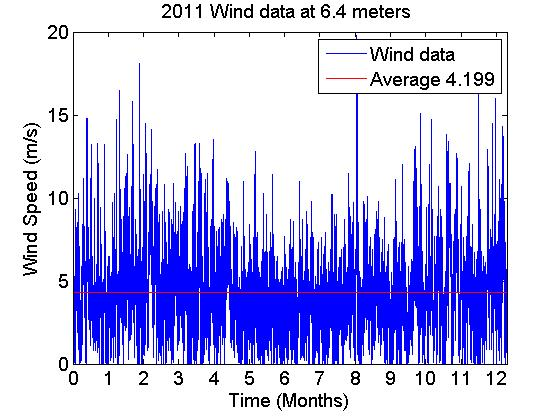
\includegraphics[width=\linewidth]{blum_figure1}
\caption{\textit{2012 NOAA Wind Data at 6.4 meters}}
\label{fig:new_wind_data}
\end{figure}

\begin{figure}
\centering
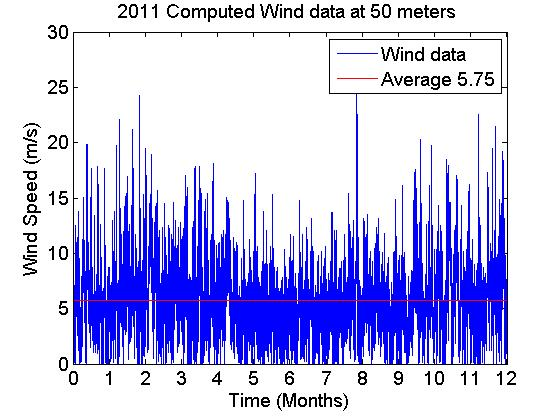
\includegraphics[width=\linewidth]{blum_figure2}
\caption{\textit{Computed 2012 NOAA Wind Data at 50 meters}}
\label{fig:new_computed_wind_data}
\end{figure}


The computed wind data was then analyzed and a probability density graph of the wind speed what created in MATLAB. Figure \ref{fig:Probality_density_function} shows a probability density graph.



\begin{figure}
\centering
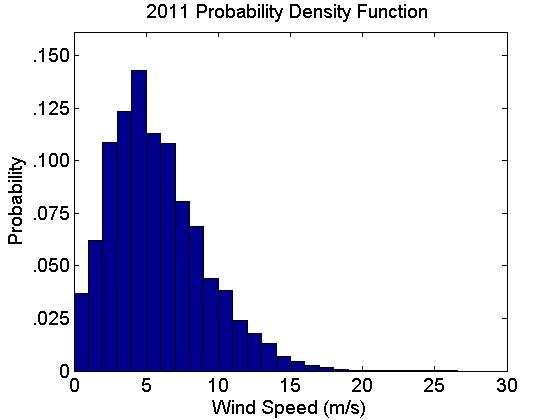
\includegraphics[width=\linewidth]{blum_figure3}
\caption{\textit{Probability Density Graph of Computed Data}}
\label{fig:Probality_density_function}
\end{figure}

The probability density graph gives a more accurate calculation of the power output. This is because the equation for power is: 

\begin{equation}
Power(W)={SA}*{AD}*{E}*{0.5}*{V^3}
\end{equation}

Where $SA$ is the swept area of the turbine blade, $AD$ is the air density, and $E$ is the efficiency of the turbine. $(0.5 * V3)$ is Velocity participating in a calculation of Kinetic Energy to produce the mass of air on the turbine \cite{ArcGIS2012}. Since Velocity is cubed in this equation, doubling the wind speed would increase the power output by eight. This is why a probability density graph is better than just a yearly average.  Also if the radius of the turbine is doubled the power output would increase by four.\\
\indent
Since the turbine will be exposed the elements of the Newport Bridge a marine grade wind turbine was necessary for this application. The wind turbine that we choses was the Sunforce 44444 12-Volt 400 Watt Wind Generator. The radius of the turbine is .56 meters. This gives a swept area of approximately .98 m2. The maximum efficiency of any wind turbine can only be 59.3 \% due to the Betz limit but this wind turbine is closer to 40\%. \cite{Windpower2008}.\\
\indent   
With the power equation, turbine efficiency, and the probability density graph, an approximation can be made about the power output from the NOAA data. The hourly output can be plotted and the cumulative annual output can be calculated. Shown in Figure \ref{fig:Hourly output in watts} and Figure \ref{fig: Cumlative power} respectfully. For this turbine at this location the total output power was calculated to be around 710,000 Watt hours. \\
\indent

\begin{figure}
\centering
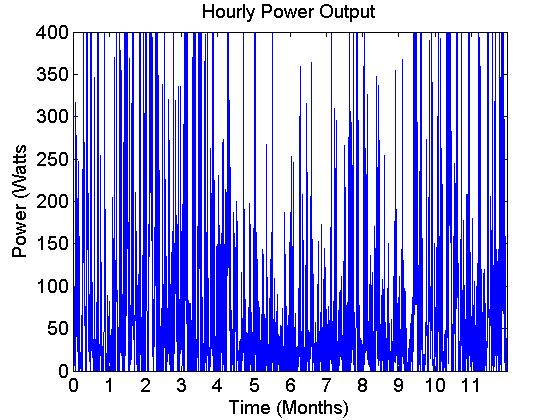
\includegraphics[width=\linewidth]{blum_figure4}
\caption{\textit{Hourly watt output}}
\label{fig:Hourly output in watts}
\end{figure}


\begin{figure}
\centering
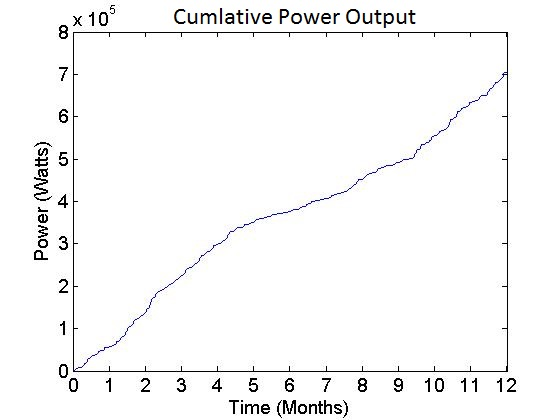
\includegraphics[width=\linewidth]{blum_figure5}
\caption{\textit{Cumulative power}}
\label{fig: Cumlative power}
\end{figure}

From the NOAA data and the wind turbine we can determine the longest time there will be no output of the turbine. This is because the cut-in speed for this turbine is 3.2 meters per second. This will help to determine the battery size. 

\begin{table}
\centering
\begin{tabular}{|l|l|l|l|l|l|l|l|}\hline
Year & 2007 & 2008 & 2009 & 2010 & 2011 & 2012 &2013\\\hline
Hours & 175 & 263 & 219 & 243 & 103 & 664 & 110\\\hline
Days & 7.3 & 10.9 & 9.1 & 10.1 & 4.3 & 27.6& 4.5\\\hline
\end{tabular}
\caption{\textit{Time without power production}}
\label{tab:widgets}
\end{table}

